\section{\tool}
\label{sec:design}

\ignore{
\subsection{Goals}
\label{sec:tool:goals}

We identify the broad design goals for a technique to automatically repair
malformed strings or incorrect handling of strings as follows:

% i) identifies the statements which might be vulnerable to string-related errors,
% and are less critical to the functionality of the application such that
% suboptimal behavior might be acceptable,
% iii) generates patches by identifying constraints on the string data and if
% required, tweaks \code{String} API  parameters to regenerate legally correct
% string data,
% iv) optimizes the number of statements to be patched by retaining only the ones
% that need to be protected,  

\myparagraph{(i) High patch fidelity} We require that the patched program must
preserve the intended program behavior, \ie\ the patch must be precise, and
should not induce any undesirable control flows in the repaired program.

\myparagraph{(ii) Non-invasive instrumentation} We require that the technique
must ensure no side-effects (aside from optimally repairing objects) during
normal program execution, and activate patches only when the program is
guaranteed to crash.

\myparagraph{(iii) Low system overhead} We desire that the patched program must
incur no runtime overhead during normal program execution, and only negligible
overhead in case of failures.
}

% \subsection{Design}
% \label{sec:tool:design}

\begin{figure}[t]
\centering
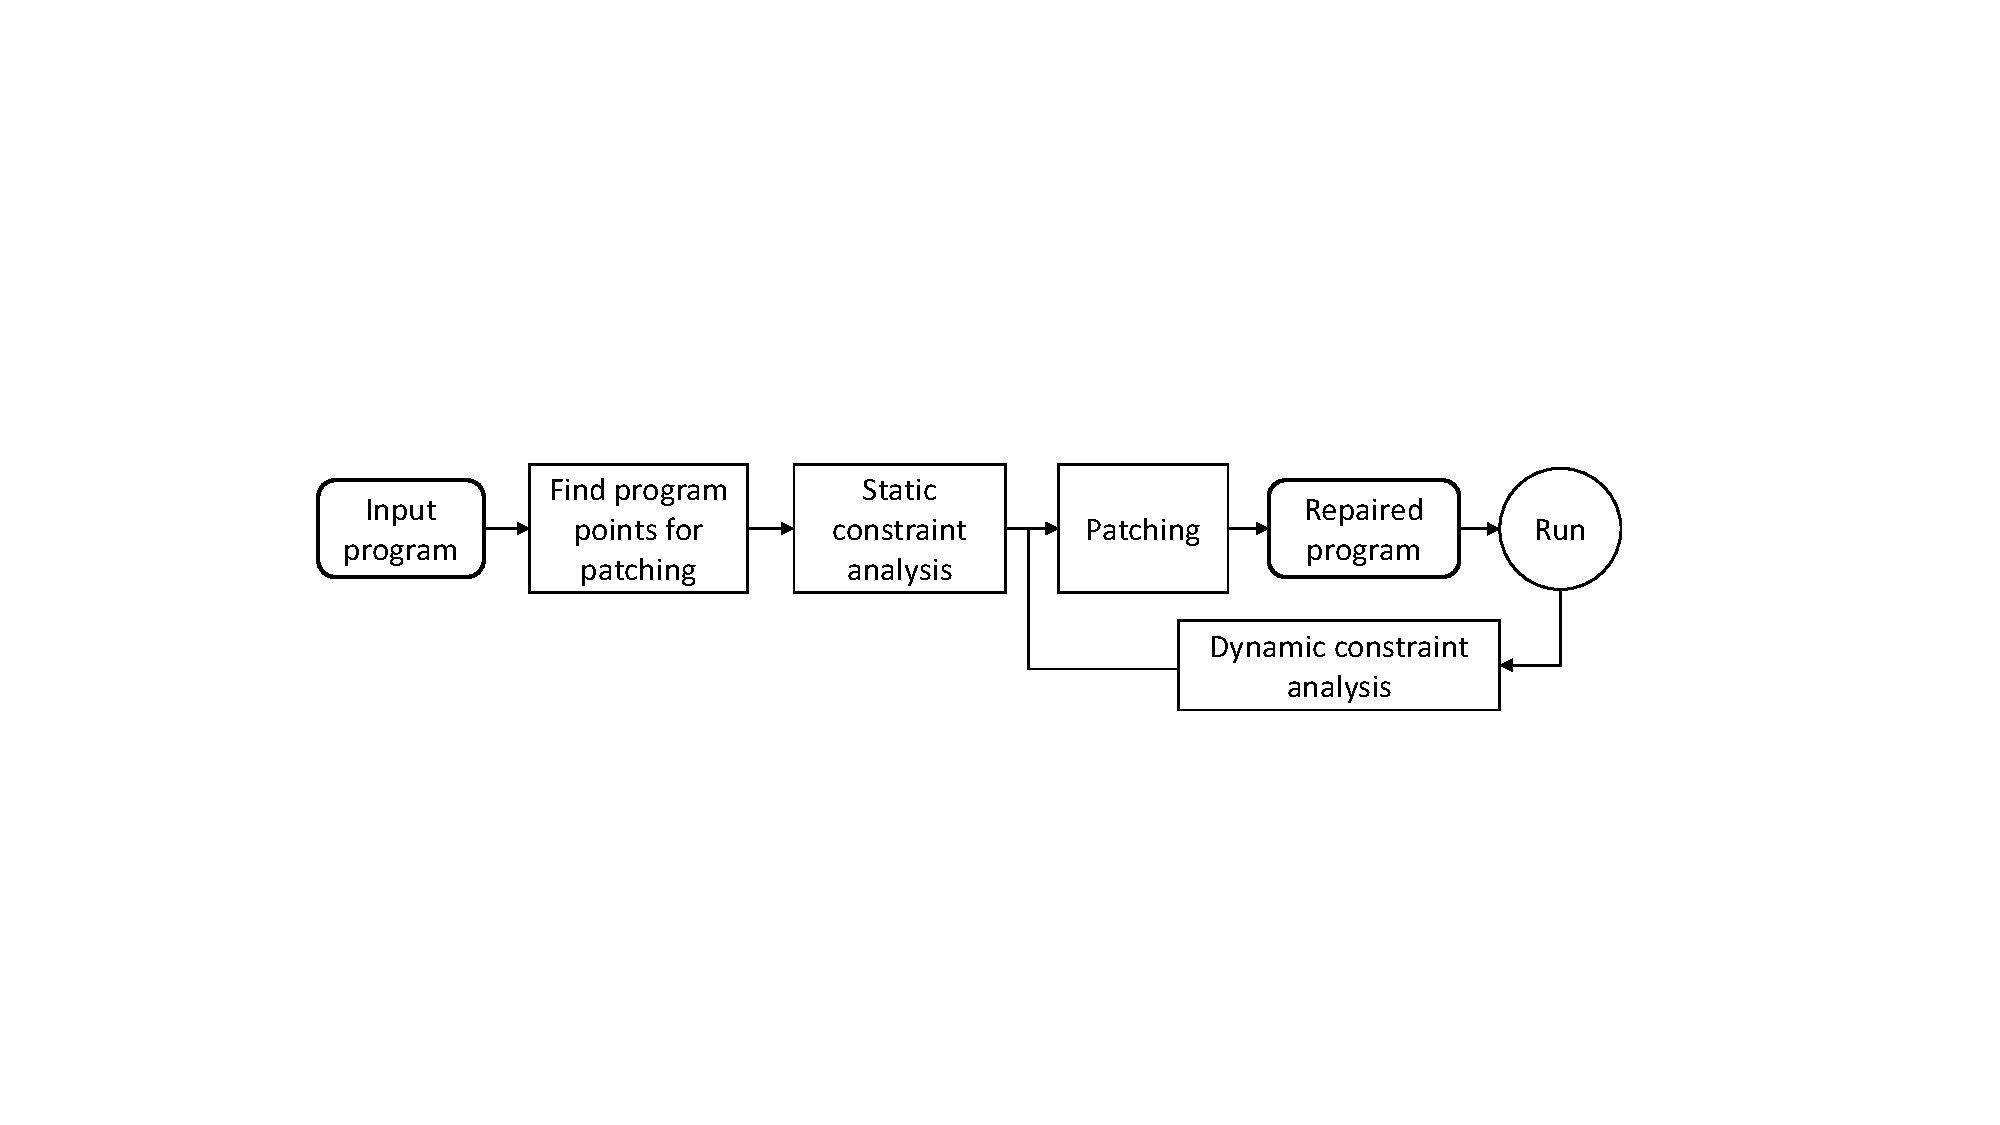
\includegraphics[scale=.38]{images/NewDesignDiagram.pdf}
\caption{\tool\ workflow.}
\label{fig:overallDesign}
\end{figure}

\myparagraph{\underline{Key Idea}} \tool\ leverages a combination of program 
analysis techniques to precisely identify program instrumentation points, and
builds upon custom algorithms to generate targeted, high quality patches for
repairing programs with potential runtime exceptions, while still satisfying
goals mentioned in \xref{sec:tool:goals}.

Figure~\ref{fig:overallDesign} shows \tool's workflow, which involves three
main stages. First, \tool\ uses program analysis techniques to precisely
identify points of interest, \ie\ string objects or API arguments that must be
repaired to prevent runtime exceptions. In the second stage, \tool\ leverages
custom algorithms to generate relevant patches. Specifically, \tool\ performs
intra-procedural static and dynamic analyses to identify and evaluate
constraints on the string objects under consideration. Third, \tool\ uses the
constraints evaluated in the earlier stage to programatically generate and embed
patches inside \texttt{catch} blocks to ensure that they do not get activated
during normal program execution.

\subsection{Precise Identification of Instrumentation Points}
\label{sec:tool:stage1}

In this stage, \tool\ leverages a combination of program analyses to accurately
determine the minimum set of points of interest where instrumentation is
required to repair. We list several techniques below that help \tool\ achieve
precision.

\myparagraph{(i) Taint analysis} The main purpose of taint analysis is to
broadly identify which program statements can be patched (possibly even
suboptimally) without affecting the program control flow, \ie\ affect only
objects that are generated and stay within the application throughout their
lifetime. While this principle is not a binding constraint, it ensures that
\tool's repairing mechanism does not adversely affect critical program behavior.
We specify a generic set of sensitive sources and sensitive sinks for each input
program, to identify critical program paths where a repaired \code{String}
objects (and thus possibly suboptimal) must not flow. For example, \tool\ does
not repair program statements that lie along a control flow path that leads to
an I/O sink, like file system, console, network, GUI, etc.

\begin{table}[t]
\centering
\scriptsize
% \setlength{\tabcolsep}{3pt}
% \hrule
\begin{tabular}{|l|l|}
\hline
\multicolumn{1}{|c|}{\textbf{Class}} & \multicolumn{1}{c|}{\textbf{Source}}\\
\hline
\code{java.io.InputStream} & \code{read()}\\
\code{java.io.BufferedReader} & \code{readLine()}\\
\code{java.net.URL} & \code{openConnection()}\\
\code{java.util.Scanner} & \code{next()}\\
% \code{javax.servlet.http.HttpServletRequest} & \code{getParameter()}\\
\code{javax.servlet.ServletRequest} & \code{getParameter()}\\
\code{org.apache.http.HttpResponse} & \code{getEntity()}\\
\code{org.apache.http.util.EntityUtils} & \code{toString()}\\
\code{org.apache.http.util.EntityUtils} & \code{toByteArray()}\\
\code{org.apache.http.util.EntityUtils} & \code{getContentCharSet()}\\
\hline
\end{tabular}
\caption{Common sensitive sources in \java.}
\label{table:TaintSources}
\end{table}

\begin{table}[t]
\centering
\scriptsize
% \setlength{\tabcolsep}{3pt}
\begin{tabular}{|l|l|}
\hline
\multicolumn{1}{|c|}{\textbf{Class}} & \multicolumn{1}{c|}{\textbf{Sink}}\\
\hline
\code{java.io.FileOutputStream} & \code{write()}\\
\code{java.io.OutputStream} & \code{write()}\\
\code{java.io.PrintStream} & \code{printf()}\\
\code{java.net.Socket} & \code{connect()}\\
\code{java.io.Writer} & \code{write()}\\
\hline
\end{tabular}
\caption{Common sensitive sinks in \java.}
\label{table:TaintSinks}
\end{table}

The taint analysis module takes as input the compiled byte code intended to be
repaired, and generates a control flow graph identifying program statements that
lie along paths from sensitive sources to sensitive sinks. Since, \tool\ targets
strings in particular, it must support taint propagation for all \java\ APIs
that support string manipulation, including \code{StringBuffer} and
\code{StringBuilder}. All \code{String} objects (whether generated or assigned)
that lie along the tainted path from a sensitive source to a sensitive sink are
marked as \textit{unsafe} to patch. Subsequently, \tool\ does not repair such
\code{String} objects. Tables~\ref{table:TaintSources} and
\ref{table:TaintSinks} list some common sensitive sources and sinks for several
classes in \java. \comment{Can we make exceptions to these?}

\myparagraph{(ii) Call graph analysis} \tool\ leverages call graph analysis to
further improve the precision for finding instrumentation points. Although
unlikely, it is possible that the developers may themselves handle code that
raises runtime exceptions. Thus, \tool\ must not instrument program points that
are explicitly handled by the developers, since repairing such statements
would definitely alter the intended control flow.

Checked runtime exceptions may be placed in the (i) same method, or (ii)
upstream in the call chain. While handling the former scenario is trivial,
\tool\ handles the latter case by identifying all possible call chains (in
the call graph) involving the concerned method using reverse Breadth First
search (BFS), and determines ancestor methods where the call site was wrapped in
\code{try-catch} block of compatible exception type or not.

\myparagraph{(iii) Reaching definitions analysis} Taint and call graph analyses
together provide a set of program points to be instrumented with the
patch. However, this set can be further pruned. \tool\ performs \textit{reaching
definitions} analysis to skip marked statements if
(i) the string variables contained in such statements have already been patched
upstream in the method, and (ii) the variables have not been redefined along any
path that originates from the patched statement. This analysis further reduces
instrumentation points in a program.

\subsection{Patch Generation}
\label{sec:tool:stage2}

The output from the first stage is essentially a set of program points,
typically bytecodes or some other intermediate representation, denoting
\code{String} objects or APIs that are safe to repair. Once these
instrumentation points have been identified, \tool\ determines the
possible patches that can be applied to each of them. Specifically, a program
patch constitutes a set of constraints on either the \code{String} object or the
parameters to the \code{String} API under consideration, such that the new
repaired \code{String} object that is generated will satisfy all constraints and
thus the patched program does not throw any runtime exceptions.

\tool's patch generation mechanism involves two main parts (i) constraint
collection and evaluation, and (ii) code generation. We now describe \tool's
patch generation mechanism in detail. 

%
\begin{figure}[t]
\centering
%% change the font size in the img; make it min len, max len
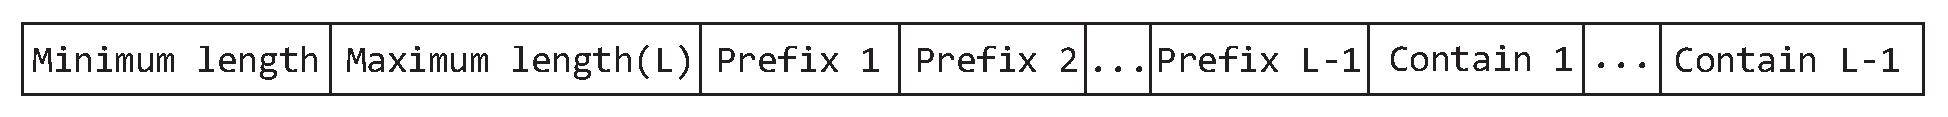
\includegraphics[width=\linewidth]{images/constraint.eps}
\caption{Constraints involving Strings.}
\label{fig:constraint}
\end{figure}
% 

\myparagraph{Constraint collection and evaluation} \tool\ leverages a hybrid
approach to collect all possible constraints that must be satisfied, and thus
generates a high quality patch to repair the program. A constraint on a string
object is defined as a set of permissible values that can uniquely define the
string. \tool\ uses a simple constraint set that includes minimum and maximum
length, along with set of permissible prefixes and substrings, as shown in
Figure~\ref{fig:constraint}.

\begin{algorithm}[t]
\scriptsize
\DontPrintSemicolon
\KwData{Control flow graph $CFG$ for program $P$}
\KwResult{Patched program $P'$}
\Begin
{
 \For{$\forall$ node $N \in CFG$} {
  Statement $S$ in node $N$\\
  \lIf{$S$ contains \code{String} API call} {\\
  	\mytab $str \longleftarrow$ \code{String} reference on $S$
  	
  	\lIf{$S$ can throw \code{RuntimeException}} {\\
  	  \mytab Exception class $EC \longleftarrow$ \code{RuntimeException} of
$S$\\
          \mytab $CES_{str} \longleftarrow$ all conditional statement in $P$ on
$str$\\
  	  \mytab $CS_{str} \longleftarrow$ output of
Algorithm~\ref{algo:constraintCollection}$(CES_{str})$\\

  		\mytab \lIf{$str$ have sufficient constraints in $CS_{str}$} {\\
			\mytab \mytab \code{/* Static constraint analysis */}\\
  			\mytab \mytab $str \longleftarrow$ output of
Algorithm~\ref{algo:constraint}$(CS_{str})$
  		} \mytab \lElseIf {$str$ encountered exception} {\\
  		        \mytab \mytab \code{/* Dynamic constraint analysis */}\\
  		        \mytab \mytab $CS_{str} \longleftarrow$ output of
Algorithm~\ref{algo:constraintCollection}$(CES_{str})$\\

                        \mytab \mytab \lIf{$str$ have sufficient constraints in
$CS_{str}$} {\\
                        \mytab \mytab \mytab $str \longleftarrow$ output of
Algorithm~\ref{algo:constraint}$(CS_{str})$
  		} \mytab \mytab \lElse {\\
  		        \mytab \mytab \mytab $str \longleftarrow$ output of
Algorithm~\ref{algo:stringPatchParametr}$(S)$
  		}\vspace{-4em}
	}
    }
  }
 }
}
\caption{Patching strategy for \code{String} objects.}
\label{algo:patchingStrategy}
\end{algorithm}

The hybrid approach has a static component that makes a forward pass over the
program to collect declarative constraints on string objects, such as their
length or prefix, etc. \tool\ invokes the dynamic component if there are constraints
such that the constraint set cannot be evaluated. In
such scenarios \tool\ (i) generates a patch that itself dynamically collects
constraint information, (ii) augments it with the previously collected static
constraint details, and (iii) evaluates these constraints on the fly to generate
repaired \code{String} objects, which do not cause the program to throw runtime
exceptions. Algorithm~\ref{algo:patchingStrategy} gives an overview of this
hybrid approach.

\begin{algorithm}[t]
\scriptsize
\DontPrintSemicolon
\KwData{Set of conditional statement on string $str$}
\KwResult{Constraint set $CS_{str}$}
\Begin
{
  \For{Conditional statement$ \leftarrow i$, $\forall i \in CS_{str}$}
  {
   $i \Rightarrow str\ *\ OP$ \code{/*where $*$ is the binary operator*/}\\
   \lIf{$*$ is $==$} {\\
   \mytab $maxlength_{str} \longleftarrow OP$\\
   \mytab $minlength_{str} \longleftarrow OP$
   } \lElseIf {$*$ is $\textgreater$ {\bf OR} $*$ is $\ge$} {
    $minlength_{str} \longleftarrow OP$
   } \lElseIf {$*$ is $\textless$ {\bf OR} $*$ is $\le$} {
    $maxlength_{str} \longleftarrow OP$
   } \lElseIf {$*$ is Prefix Check} {
    $\textit{PrefixSet}_{str} \cup OP$
   } \lElseIf {$*$ is Contains Check} {
    $\textit{ContainSet}_{str} \cup OP$
   }
  }
}
\caption{Constraint collection for \code{String} objects.}
\label{algo:constraintCollection}
\end{algorithm}

\begin{mylist}

 \item \textbf{Static constraint collection}: \tool's static constraint
collection phase identifies all declarative constraints.
Algorithm~\ref{algo:constraintCollection} briefly describes the steps to
populate the constraint store shown in Figure~\ref{fig:constraint}.
Specifically, \tool\ iterates over all program code and analyzes conditional
statements involving string objects of the form \code{if (st.length() == $5$)}.
\tool\ considers only those constraints that the object must satisfy to ensure
that the control flows through the \textit{preferred} branch of the conditional.
We define the preferred branch as the one that does not throw exceptions or
error conditions, like \code{System.err.print()}. In other words, \tool\ only
considers the conditional expressions in the branches that do not involve any
exceptions or error paths. Note that \tool\ also evaluates $OP$ (in
Algorithm~\ref{algo:constraintCollection}) when collecting constraints, in case
$OP$ is a composite mathematical expression $f(x,y,z,...)$, such as $x + y * z$,
where all $x$, $y$ and $z$ are known to be numeric.

\begin{algorithm}[t]
\scriptsize
\DontPrintSemicolon
\KwData{String object \textit{Str} and constraint set $CS$.}
\KwResult{String object \textit{Str} such that $\forall i \in CS$, $Str$ satisfies $i$}
\Begin {
    $CS_{\textit{Str}} \longleftarrow$ Get the constraint set for \textit{Str}\\
    $MinLength \longleftarrow CS_{\textit{Str}}[0]$\\
    $MaxLength \longleftarrow CS_{\textit{Str}}[1]$\\
    $\textit{PrefixSet}_{\textit{Str}} \longleftarrow CS_{\textit{Str}}[2 \rightarrow MaxLength + 1]$\\
    $\textit{ContainSet}_{\textit{Str}} \longleftarrow CS_{\textit{Str}}[MaxLength +2  \rightarrow
2*MaxLength + 1]$\\

    \For{$C \in \textit{PrefixSet}_{\textit{Str}}$} {
        \lIf{$C$ is Empty} {\\
          \mytab continue
        }
        
        $\textit{PrefixLength} \longleftarrow$ {\bf LENGTH OF} $C$\\
        
        \lIf{\textit{PrefixLength} is Maximum $\in \textit{PrefixSet}_{\textit{Str}}$} {\\
          \mytab  Use $C$ to construct $\textit{Str}$
        }
    }

    \For{$C \in \textit{ContainSet}_{\textit{Str}}$} {
        \lIf{$C$ is Empty {\bf OR} $C \in \textit{Str}$} {\\
          \mytab  continue
        }
        $\textit{Str} \leftarrow \textit{Str}$ {\bf APPEND} $C$
    }
    return $\textit{Str}$
}
\caption{String object constraint evaluation.}
\label{algo:constraint}
\end{algorithm}

 \item \textbf{Dynamic constraint collection}: The constraint set is populated
at the end of the static phase, and \tool\ leverages
Algorithm~\ref{algo:constraint} to evaluate these constraints and determine the
potential safe values of the string object under consideration. However, there
are scenarios, where there are potentially conflicting constraints or no
permissible values of the constraints can be calculated statically.

\lstset{language=Java, caption=Code requiring dynamic string constraint
evaluation., label =
snippet:exCode1, firstnumber =1}
\begin{figure}[t]
\begin{lstlisting}
void foo() {
  String st = Input(); /* user input */
  if (st.length() == 5) {/* do something */}
  if (st.contains(Input())) {/* do something */}
  st = st.substring(7, 10);
}
\end{lstlisting}
\end{figure}

\lstset{language=Java, caption=Dynamic constraint collection and evaluation
corresponding to code \ref{snippet:exCode1}., label =snippet:exCode2,
firstnumber =1}
\begin{figure}[t]
\begin{lstlisting}
String temp = Input();
ConstraintStore.updateSet("<foo()>", st, temp);
st = GenerateStringDynamic.init("<foo()>", st);
\end{lstlisting}
\end{figure}

Consider the example shown in Code~\ref{snippet:exCode1}, where the function
\code{foo} performs a series of checks on a user-entered string \code{st} before computing
a substring on it. Since the constraints on \code{st} cannot be
completely collected and evaluated statically. For such cases, \tool\
instruments the code with statements to dynamically collect constraint
information, augment them with previously known static constraints, and evaluate
these constraints at runtime. Specifically, \tool\ instruments the bytecode
with constraint collection code just before the conditional statements under
consideration. Thus, \tool\ will insert Code~\ref{snippet:exCode2} before line
$4$ in Code~\ref{snippet:exCode1} to update and evaluate the set of constraints
on string \code{st}.

\end{mylist}

\subsection{Code generation}
\label{sec:tool:stage2:generation}

Code generation is done either statically or dynamically depending on how
the constraints are evaluated. In either scenario, a key component of code
generation is \textit{object repairing}. Additionally, in certain cases
where constraints cannot be satisfied, either statically or dynamically or
both, \tool\ resorts to \textit{parameter tweaking}.
%The mechanism by which \tool\ achieves this is primarily based on 
%\textit{parameter tweaking}.

\begin{mylist}

 \item \textbf{Object repairing}: \tool\ generates the code for the repaired
object under consideration after all the constraints have been collected and
evaluated. If the constraints are resolved statically, then \tool\ updates its
constraint data store and instruments the corresponding bytecodes appropriately.
However, in case the patch requires dynamic constraint collection, \tool\ embeds
the code to dynamically collect constraints and generate the patch as well. Line
$1$ and $3$ in Code~\ref{snippet:exCode2} update the constraint set and generate
the repaired object, respectively.

\begin{algorithm}[t]
\scriptsize
\DontPrintSemicolon
\KwData{String object \textit{Str} and index set $IS$ which contains ${i}$ or ${i,j}$.}
\KwResult{Repaired index set containing ${R_i}$ or ${R_i,R_j}$ based on input $IS$}
\Begin {
    $Length \longleftarrow$ length of \textit{Str}
    
    \lIf{$Length == 0$} {\\
     \mytab $R_i, R_j \longleftarrow 0$
    } \lElse {
        \lIf{$i \textgreater j$} {\\
           \mytab $R_i \longleftarrow j - 1$
        }
        \lIf{$i \textgreater Length$ \bf{OR} $j \textgreater Length$} {\\
           \mytab $R_i \longleftarrow Length - 1$ or $R_j \longleftarrow Length -
1$ based on condition\\
           \mytab \code{/* more conditions possible */}
        }
        \lIf{$i \textless 0$ \bf{OR} $j \textless 0$} {\\
          \mytab $R_i \longleftarrow 0$ or $R_j \longleftarrow 0$ based on
condition\\
          \mytab \code{/* more conditions possible */}
        }\vspace{-1em}
    }
}
\caption{Parameter tweaking based String patching.}
\label{algo:stringPatchParametr}
\end{algorithm}

\lstset{language=Java, caption=Example of parameter tweaking.,
label =
snippet:exCode3, firstnumber =1}
\begin{figure}[t]
\begin{lstlisting}
try{
    c = s.chatAt(4);
} catch(IndexOutOfBoundException ex) {
    c = s.failSafeCharAt(4, s.length());
}
\end{lstlisting}
\end{figure}

 \item \textbf{Parameter tweaking}: It is possible that as a side-effect of
object repairing, the newly patched object may throw runtime errors when
invoked with certain string APIs. For example, \code{c = s.charAt(4);} may still
throw runtime errors even if \code{s} has been repaired. This is possible if
the repaired \code{s} has a length less than $4$. In such scenarios, \tool\
patches the code with a \code{try-catch} block around the offending API call,
and appropriately inserts the repaired code in the \code{catch} block but with
tweaks to the API arguments, as shown in Code~\ref{snippet:exCode3}, to ensure
that no further runtime exception is thrown. For example, if the length of the
string is greater than $4$, then the API works similar to default \code{charAt}
API. However, if the length is $3$, then line $4$ is invoked with both arguments
equal to string length, \ie\ $3$. Note that parameter tweaking is leveraged to
counter a potentially suboptimal object repair that may throw cascading
exceptions. Algorithm~\ref{algo:stringPatchParametr} briefly outlines
the mechanism to correctly set the parameters for the offending string API.

\end{mylist}

\subsection{Instrumentation}
\label{sec:tool:stage3}

\tool\ embeds the repair in a \code{try-catch} ladder to ensure that the patches
do not get activated during normal program execution, thereby minimizing any
side-effects of repairing and preventing any inadvertent changes to the
program's intended control flow.

An important task in the instrumentation stage is to determine the kind of
exceptions that may be thrown, and appropriately construct the \code{catch}
blocks. While most APIs throw only a single subclass of \code{RuntimeException},
it is possible that a statement may throw more than one subclasses, such as
\code{NullPointerException} and \code{StringIndexOutOfBoundsException}. \tool\
generates a \code{catch} ladder for each kind of exception, which also
facilitates exception-specific repairing as well. In other words, a single patch
may get distributed over multiple \code{catch} blocks. This mechanism is
achieved with the help of a constraint representation model.

%-------------------

\myparagraph{Constraint representation model}  We use a finite state
machine
(FSM) as a formalism to describe the behavior of \java\ \code{String} API, and 
apply it to drive the generation of exception-specific \code{catch} blocks. The
model is precomputed based on the API documentation of \java\ \code{Strings}.
Formally, we define the constraint representation FSM model $(Q, \Sigma, \delta,
q_0, F)$ as follows:
\begin{mybullet}
 \item $Q$: Set of states where $|Q| = 2$, \emph{legal state}(safe) and
\emph{illegal state} (error).

 \item $\Sigma$: Set of symbols. Each symbol is defined as a tuple ($\zeta$,
$\eta$, $\Lambda$), where $\zeta$ is a \code{String} API operation, $\eta$ is
the type of an exception and $\Lambda = \{\lambda_1, \ldots, \lambda_n\}$  is
the set of constraints. A constraint $\lambda_i$ is defined as a constraint on
a string that must be satisfied to allow successful execution of $\zeta$.

 \item $\delta$: Transition function. $safe \rightarrow safe$ is a safe
transition and $safe \rightarrow error$ corresponds to the constraint violation.

 \item $q_0$: Starting state, here $q_0 = safe$.

 \item $F$: Singleton set of accept states which contains $q_0$.
\end{mybullet}

\begin{figure}[t]
\centering
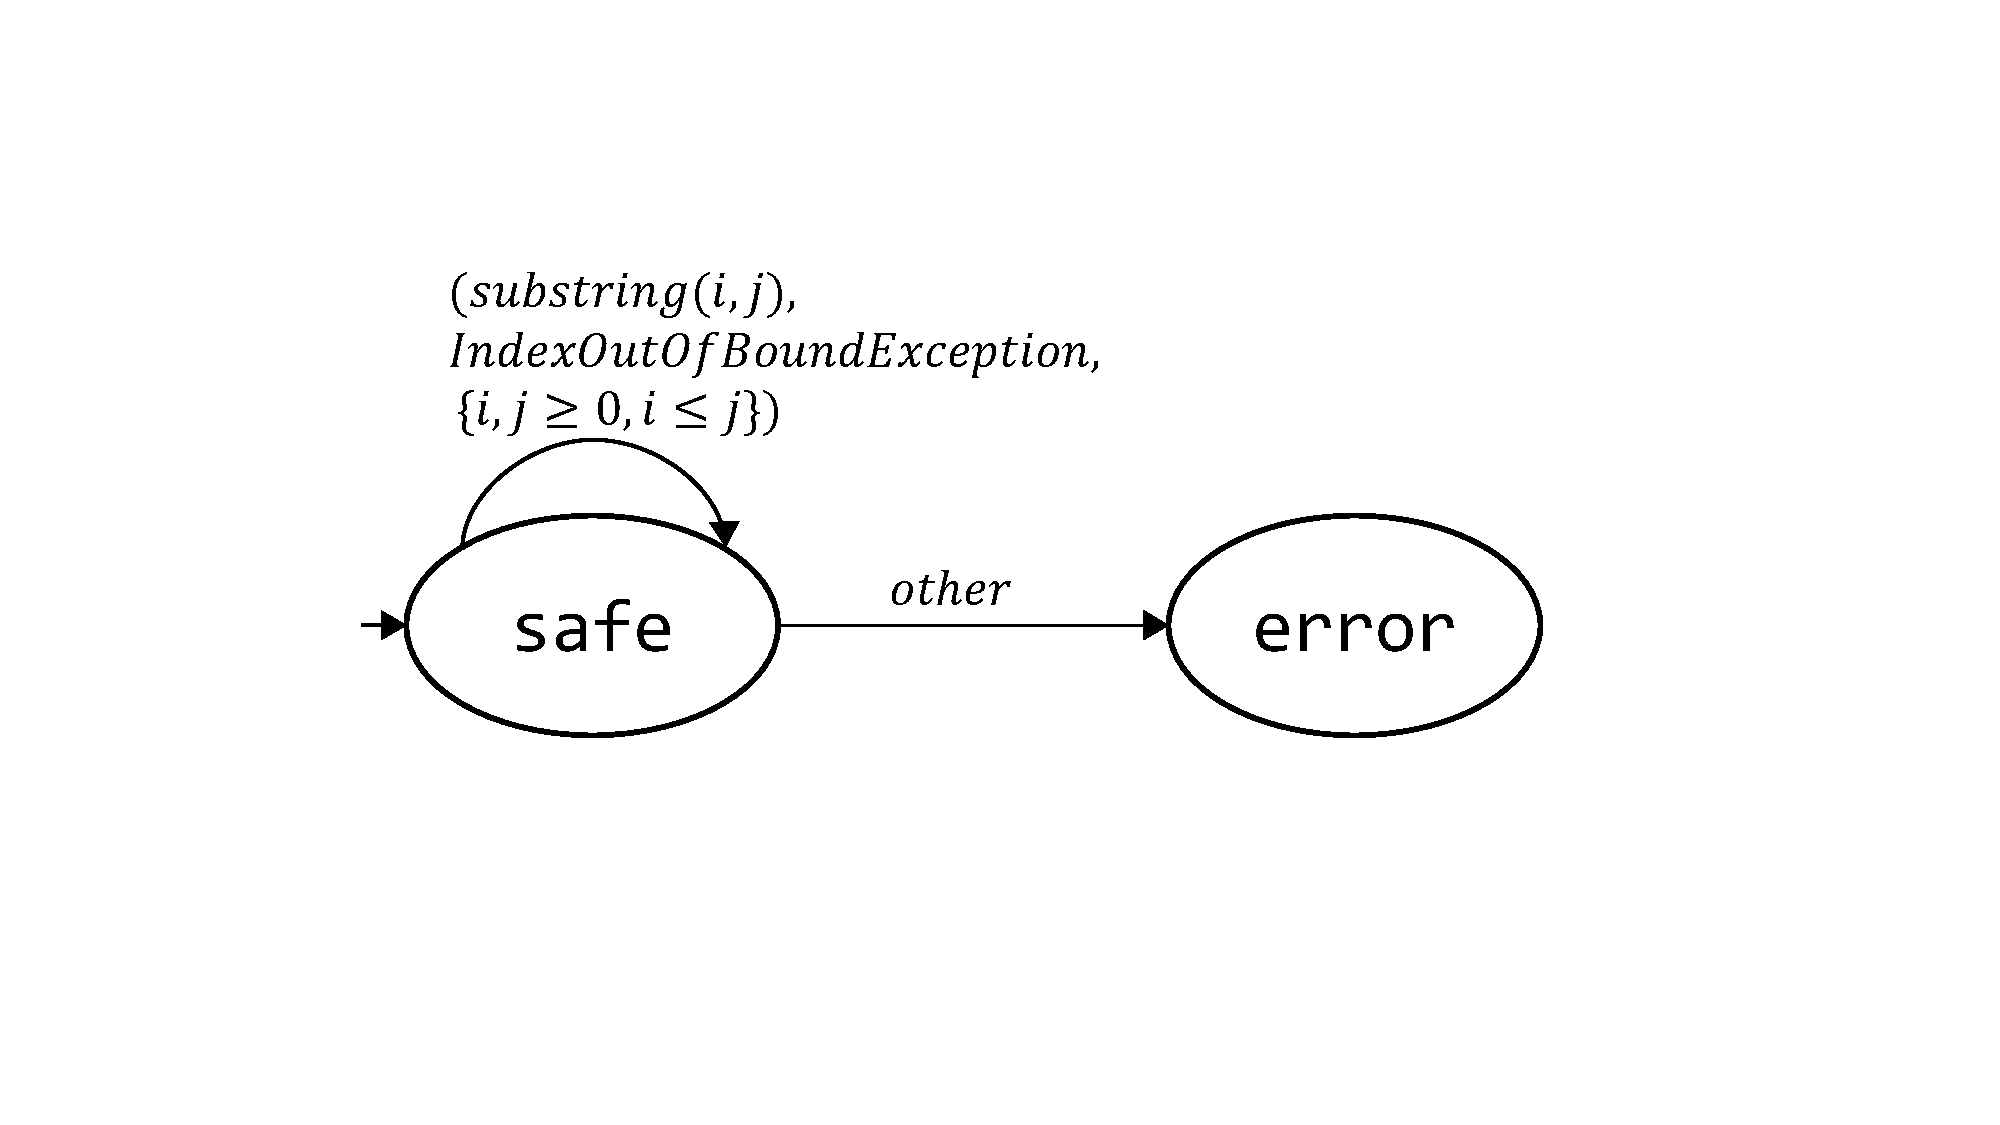
\includegraphics[scale=.25]{images/automataString.pdf}
\caption{Partial constraint representation model.}
\label{fig:constraintautomata}
\end{figure}

% An abstract constraint representation model is depicted in
% Figure~\ref{fig:constraintautomata}. A concrete model be constructed using an
% exception-specific information that is available in the API documentation. The
% repairing mechanism gets triggered when some $\eta$ is thrown while performing
% $\zeta$ after at least one of the constraints from $\Lambda$ on the structure of
% the associated string is violated. The patches essentially support the same
% semantics using multiple \code{catch} blocks corresponding to various
% exceptions.


A partial constraint representation model is depicted in
Figure~\ref{fig:constraintautomata}. It essentially specifies the constraints
that are associated with \code{substring}
method and \code{IndexOutofBoundException} exception that can be thrown by the
method. A complete model would
have several such self-looping transitions corresponding to other \java\
\code{String} API methods. The
repairing mechanism gets triggered when an exception is thrown while performing
a string operation after at least one of the constraints on the structure of
the associated string is violated. This is represented by the transition labeled
by \code{other}. The patches essentially support the same
semantics identified by the transitions with the help of \code{catch} blocks.

%------------------------

\subsection{Limitations}
\label{sec:tool:limitation}

\tool's major limitation arises from the fact that it
is heavily directed towards repairing handling \code{String} objects and API
exceptions. While this may seem to be a limitation, we believe that \tool's
strength lies in the fact that it mines contextual data about runtime exceptions
related to \code{String} objects that helps development of intelligent program
patches. Moreover, \tool's technique is generic and can be ported to any other
class of \java\ APIs.

\tool generates precise patches considering the program context which avoids
cascading exceptions to a great extent producing the intended behavior in case
of failures. However, it still cannot give guarantees about elimination of cascading
exceptions, particularly when there are heavy object dependencies in the program.

The quality of \tool's patches also depends on the nature of the constraint
solver, which is pluggable. A more sophisticated solver may improve the quality
of program repair, and we leave comparison of different solvers for future work.

\ignore{
\paragraph{Identifying Program Statements.} We perform static taint analysis
to identify sensitive data which are leaving the system via database, network
stream, file stream or console. Providing patches to the
statements that manipulate this data would be undesirable, since
activation of the patches in case failures may allow altered sensitive data to
eventually
reach users. Hence, we only mark those program statements which do
not manipulate these data.

\paragraph{Noninvasive Patching.} In case a runtime exception that is thrown
by a statement as a result of a failure is already caught and handled in a
program,
we skip that statement from patching to avoid interfering with the results. Such
statements are identified by analyzing call-graphs and ensuring that no caller
method
in the call-chain handles the exception or its superclass. By embedding the
patches inside
\texttt{catch} blocks, we ensure that they do not get activated during normal
program execution.

\paragraph{Patch Generation.} We first perform an
intra-procedural static analysis
to identify constraints on the string objects under consideration. By
identifying
the type of exceptions that can be thrown in case of a failure, we
develop patches that
regenerate string objects by tweaking \java\ \code{String} API used in
the statements to regenerate legal string objects and by trying to solve the
constraints. In the latter case,
we evaluate the constraints statically if complete information is available at
the compilation-time. Otherwise, the analysis automatically generates
code that performs dynamic analysis to solve the constraints, and then
inserts this code in the generated patches.

\paragraph{Optimizing Instrumentation.} We perform reaching definitions
analysis to skip marked statements
if the string variables that are contained in the statements are already
patched, and the variables
are not redefined along any path that originates from the patched statement.
This analysis reduces
instrumentation points in a program.

\paragraph{Patch Precision.} The precision of a program patch is improved,
firstly, by targeting only strings
for patching which allows us to develop more specialized patches, secondly, by
patching programs very
close to the points of potential failures which avoids unnecessary patching of
other
unaffected variables and their potential
side effects, thirdly, by analyzing the types of exceptions that can be thrown
which
provides valuable insights into
origins of failures, and finally, by considering all the constraints
on the strings. This would result
in a program behavior closed to the intended one in case of a failure.

\paragraph{Reduced Overhead.} The side-effect of non-invasive patches is that
they do not interfere during
normal execution which results in no runtime overhead. Even when they get
activated in case of failures,
they still cause negligible overhead since we perform no analysis during runtime
except if required resolve the dynamic constraints.
As our study reveals~\xref{sec:evaluation} the constraints are typically few and
simple, making
the dynamic analysis light-weight.
}

